% Author: Alfredo Sánchez Alberca (asalber@ceu.es)

\chapter{Introduction to Excel}
Excel is a spreadsheet application that is part of the Microsoft Office suite.

\begin{center}

\includegraphics[scale=0.7]{../img/excel_splash.png}
\end{center}


\section{What is a spreadsheet?}\hypertarget{what-is-a-spreadsheet}{}\label{what-is-a-spreadsheet}

A \href{https://en.wikipedia.org/wiki/Spreadsheet}{spreadsheet} is a program that allows to enter data and make calculations with them in a grid layout.

There are a lot of programs for managing spreadsheets but the most famous are \href{https://products.office.com/en/excel}{Excel}, in the Microsoft Office suite, and \href{https://www.libreoffice.org/discover/calc}{Calc}, in the LibreOffice suite. Although Calc is opensource, with all the advantages associated therewith, Excel is by far the most widespread and mature spreadsheet, thus this manual covers Excel 2010. However, some of the procedures and methods explained in this manual are also valid for Calc.

\section{Excel 2010 main window}\hypertarget{excel-2010-main-window}{}\label{excel-2010-main-window}

The figure \ref{img-excel_2010_screenshot} shows a screenshot of the Excel 2010 main window where the different parts of
the window have been highlighted.

\begin{figure}[htbp]
\begin{center}
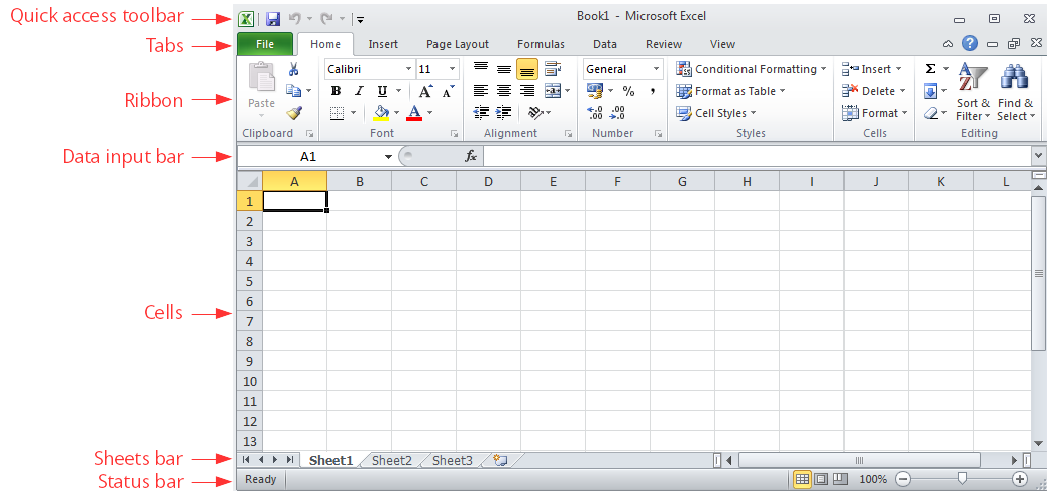
\includegraphics[max width=\linewidth]{../img/excel_2010_screenshot.png}
\end{center}
\caption{Excel 2010 screenshot.}
\label{img-excel_2010_screenshot}
\end{figure}

\section{Excel 2010 ribbon}\hypertarget{excel-2010-ribbon}{}\label{excel-2010-ribbon}

The top ribbon of Excel 2010 contains a lot of buttons that performs different actions. These buttons are arranged in panels, and panels are arranged in tabs. The main ribbon tabs are:

\textbf{File} – Performs file management tasks (new file, open file, save file, print file, etc.). It also contains general configuration options and help.

\begin{center}
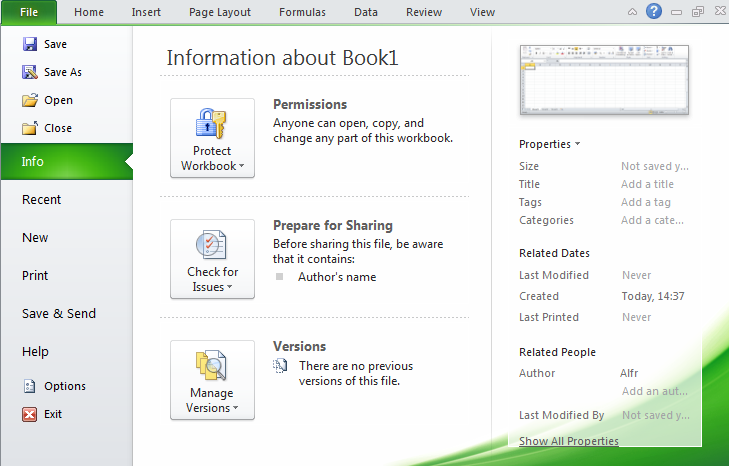
\includegraphics[max width=\linewidth]{../img/excel_2010_file_ribbon.png}
\end{center}

\textbf{Home} – Common tools (clipboard, fonts, alignment, numbers format, insert rows and columns, etc.)

\begin{center}
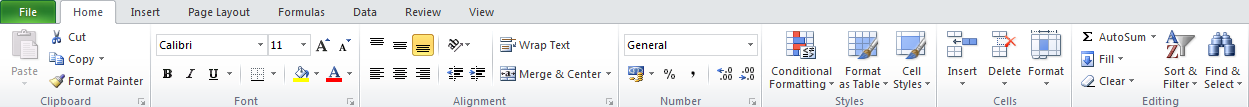
\includegraphics[max width=\linewidth]{../img/excel_2010_home_ribbon.png}
\end{center}

\textbf{Insert} – Insert objects in the sheet (tables, illustrations, charts, hyperlinks, text, equations, etc.)

\begin{center}
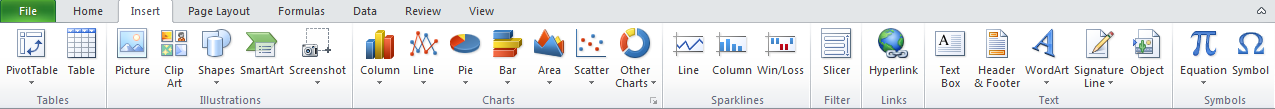
\includegraphics[max width=\linewidth]{../img/excel_2010_insert_ribbon.png}
\end{center}

\textbf{Page Layout} – Configure the printing (page setup, scale, themes, etc. )

\begin{center}
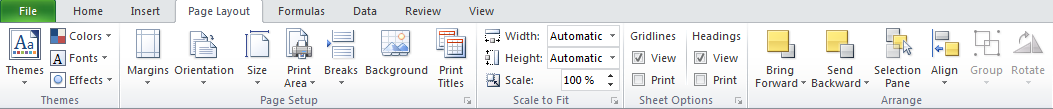
\includegraphics[max width=\linewidth]{../img/excel_2010_page_layout_ribbon.png}
\end{center}

\textbf{Formulas} – Functions arranged in categories and formula auditing.

\begin{center}
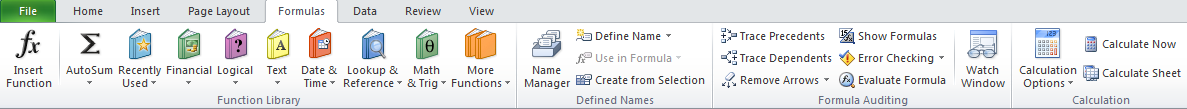
\includegraphics[max width=\linewidth]{../img/excel_2010_formulas_ribbon.png}
\end{center}

\textbf{Data} – Working with databases (import data, connection with databases, sort and filter data, data validation, etc.)

\begin{center}
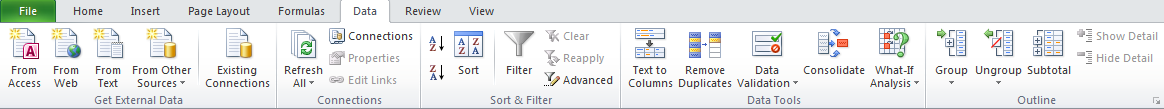
\includegraphics[max width=\linewidth]{../img/excel_2010_data_ribbon.png}
\end{center}

\textbf{Review} – Spelling, commenting, protecting and sharing sheets.

\begin{center}
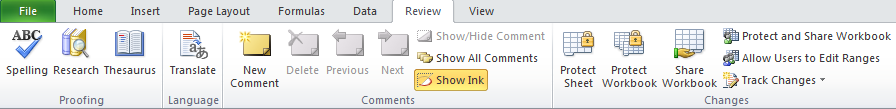
\includegraphics[max width=\linewidth]{../img/excel_2010_review_ribbon.png}
\end{center}

\textbf{View} – How Excel appears on screen (custom windows, grids lines, zoom, windows, etc. Does not affect printing).

\begin{center}
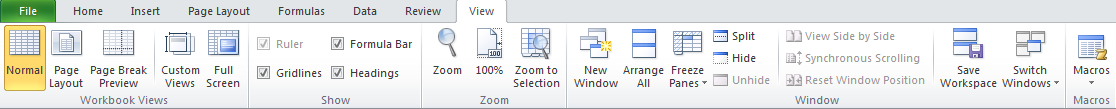
\includegraphics[max width=\linewidth]{../img/excel_2010_view_ribbon.png}
\end{center}


\subsection{Contextual tabs}\hypertarget{contextual-tabs}{}\label{contextual-tabs}

These tabs only appears in some contexts, as for example, when creating a chart or a picture.

\textbf{Chart design} Allows to select the type of chart.

\begin{center}
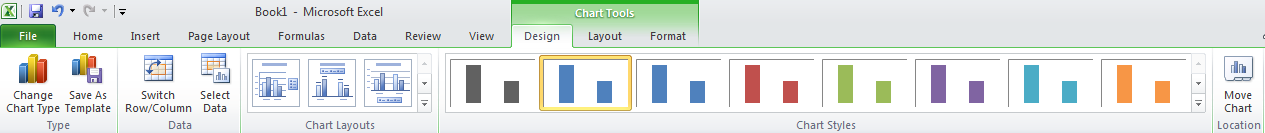
\includegraphics[max width=\linewidth]{../img/excel_2010_design_chart_ribbon.png}
\end{center}

\textbf{Chart layout} Allows to insert and configure some parts of charts (title, axis, leyend, gridlines, etc.)

\begin{center}
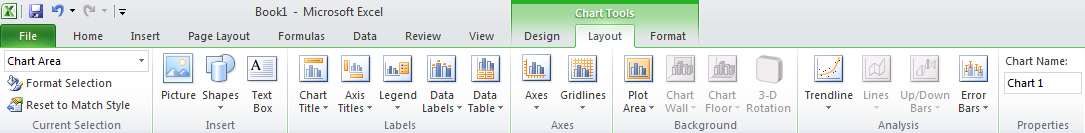
\includegraphics[max width=\linewidth]{../img/excel_2010_layout_chart_ribbon.png}
\end{center}

\textbf{Chart format} Allows to change the aspect of charts (height, width, font, colors, background, etc.)

\begin{center}
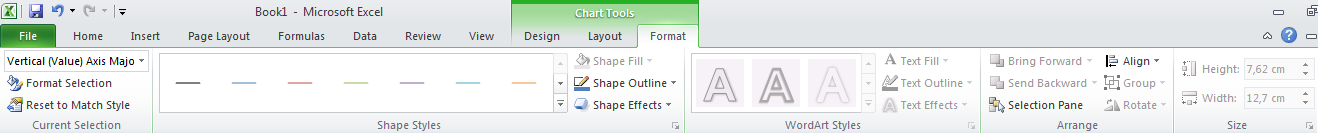
\includegraphics[max width=\linewidth]{../img/excel_2010_format_chart_ribbon.png}
\end{center}

\textbf{Picture} Allows to modify images (borders, rotation, crop, color, filters, special effects, etc.)

\begin{center}
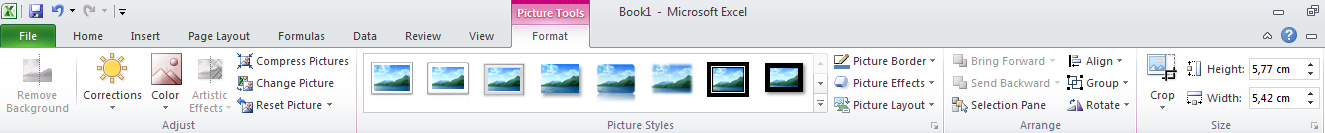
\includegraphics[max width=\linewidth]{../img/excel_2010_picture_ribbon.png}
\end{center}

In addition to these tabs, users can create their own tabs and customise them with buttons as their convenience.

There exists also a quick access toolbar just above the ribbon that can be customised with the most common buttons (see
figure~\ref{img-quick_access_toolbar}.

\begin{figure}[htbp]
\begin{center}
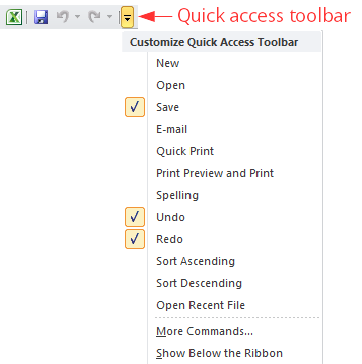
\includegraphics[max width=\linewidth]{../img/quick_access_toolbar.png}
\end{center}
\caption{Excel 2010 quick access toolbar.}
\label{img-quick_access_toolbar}
\end{figure}


\subsection{Access dialogs}\hypertarget{access-dialogs}{}\label{access-dialogs}

When you click the right bottom corner of any panel, the corresponding dialog is show where all the related options are available.

\textbf{Example}. The figure \ref{img-access_font_dialog} shows the font dialog with all the options related to fonts (font family,
font style, font size, etc.)

\begin{figure}[htbp]
\begin{center}
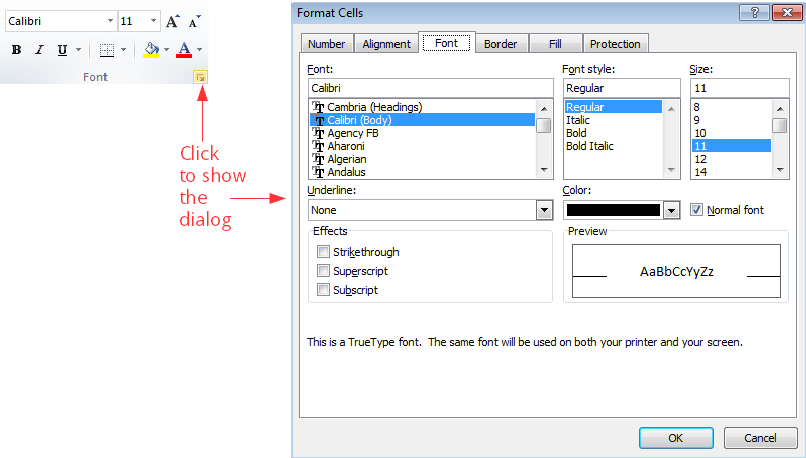
\includegraphics[max width=\linewidth]{../img/access_font_dialog.png}
\end{center}
\caption{Font dialog.}
\label{img-access_font_dialog}
\end{figure}

\subsection{Contextual menu}\hypertarget{contextual-menu}{}\label{contextual-menu}

Clicking the right button of the mouse (right-clicking) a contextual menu is showed with some buttons or options to perform actions in that context. 
This menu has different options depending on the part of the windows that is clicked.

\textbf{Example}. The figure \ref{img-contextual_menu} shows the contextual menu showed right-clicking any cell.

\begin{figure}[htbp]
\begin{center}
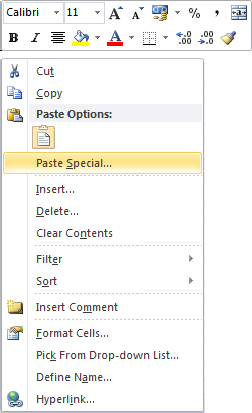
\includegraphics[scale=0.7]{../img/contextual_menu.png}
\end{center}
\caption{Cells contextual menu.}
\label{img-contextual_menu}
\end{figure}

\section{Workbooks, worksheets, rows, columns and cells}\hypertarget{workbooks-worksheets-rows-columns-and-cells}{}\label{workbooks-worksheets-rows-columns-and-cells}

An Excel file is a \emph{workbook} with several \emph{worksheets} that are two dimensional tables divided in \emph{columns} and \emph{rows}. The intersection of a column with a row is a \emph{cell} that is where data are entered. Sheets have a maximum of 16,384 columns and 1,048,576 rows.

Each worksheet has a name and are arranged in tabs at the bottom. Columns and rows have also names; columns are named with letters at the top of the column and rows with numbers to the left of the row. This way each cell is identified by the name of the worksheet, the name of the column and the name of the row where is located, and cells names follow the pattern \texttt{name-of-worksheet ! column-name row-name}. However, to refer to any cell in the active worksheet, the worksheet name may be omitted.

\textbf{Example}. The name of the selected cell in the figure \ref{img-sheet_column_row_cell} is \texttt{Sheet1!C4}.

\begin{figure}[htbp]
\begin{center}
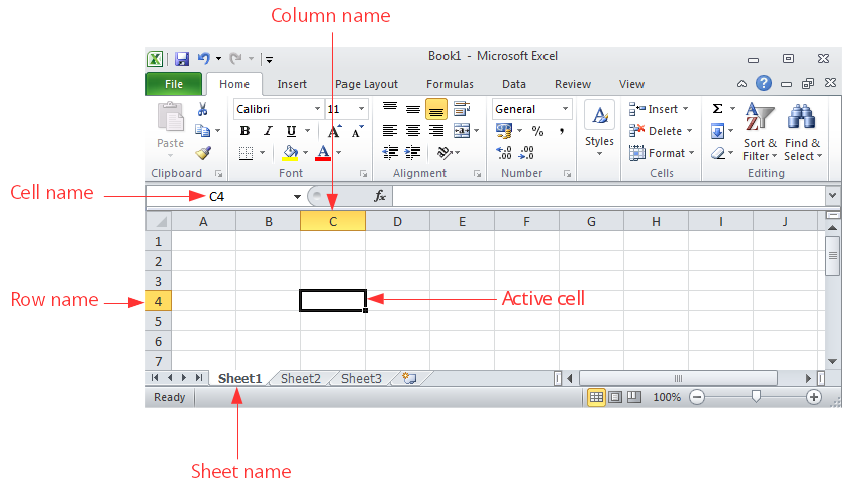
\includegraphics[max width=\linewidth]{../img/sheet_column_row_cell.png}
\end{center}
\caption{Cells, rows, columns and worksheets in Excel.}
\label{img-sheet_column_row_cell}
\end{figure}

The names of rows and columns can not be changed, but worksheet names can be changed double-clicking it and typing the new name.

\subsection{Ranges of cells}\hypertarget{ranges-of-cells}{}\label{ranges-of-cells}

A range of cells is a rectangular block of adjacent cells that is identified by top-left cell and the bottom-right cell separated by a colon, following the pattern \texttt{top-left-cell-name:bottom-right-cell-name}.

\textbf{Example}. In the figure \ref{img-cells_range} the range B3:E5 is selected.

\begin{figure}[htbp]
\begin{center}
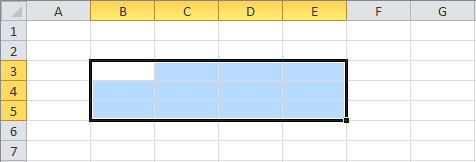
\includegraphics[max width=\linewidth]{../img/cells_range.png}
\end{center}
\caption{Range of cells.}
\label{img-cells_range}
\end{figure}

\subsection{Selecting cells, rows, columns, ranges and worksheets}\hypertarget{selecting-cells-rows-columns-ranges-and-worksheets}{}\label{selecting-cells-rows-columns-ranges-and-worksheets}

To select a cell just click it. 
To select a row click the header of the row or press the keys \texttt{Shift+Spacebar}. 
To select a column click the header of the column or press the keys \texttt{Ctrl+Spacebar}.
To select a range click one corner cell and drag the cursor over the desired cells. 
To select the whole worksheet click the top-left corner of the worksheet o press the keys \texttt{Ctrl+A}.

\textbf{Example}.  This \href{http://aprendeconalf.es/office/excel/manual/img/example_cells_selection.gif}{animation} shows how to select the cell C3, after the row 3, after the column C, after range B3:D7 and finally the whole worksheet.

\section{Data edition}\hypertarget{data-edition}{}\label{data-edition}

\subsection{Insert data}\hypertarget{insert-data}{}\label{insert-data}

Data are entered into the cells activating the cell (clicking it) and typing directly in the cell or in the input bar.

\textbf{Example}.  This \href{http://aprendeconalf.es/office/excel/manual/img/example_enter_data.gif}{animation} shows how to enter the text `Excel' in cell B2 and the number 2010 in cell C2, and after change the number of cell C2 to 2013.

Excel has a smart autocomplete feature that proposes completing the data that is typed with some predictions.

\subsection{Delete data}\hypertarget{delete-data}{}\label{delete-data}

To delete the content of a cell or a range of cells simply select the it and press \texttt{Supr} key. It's also possible to delete the cell contents with the button \texttt{Clear All}.

\subsection{Remove cells, rows, columns and worksheets}\hypertarget{remove-cells-rows-columns-and-worksheets}{}\label{remove-cells-rows-columns-and-worksheets}

To remove a whole cell (no only the content), right-click the cell and select the option \texttt{Delete...}. In the dialog that appears select \texttt{Shift cells left} if you want the cells to the left of the removed cell move to the left to fill the gap, or \texttt{Shift cells up} if you want the cells below the removed cell move up to fill the gap.

To remove a whole row, right-click the header of the row and select the option  \texttt{Delete...}.

To remove a whole column, right-click the header of the column and select the option  \texttt{Delete...}.

To remove a worksheet, right-click the tab with the name of the worksheet and select the option \texttt{Delete...}. 
\emph{Warning: Removing worksheets can not be undone!}

\textbf{Example}.  This \href{http://aprendeconalf.es/office/excel/manual/img/example_data_remove.gif}{animation} shows how to remove a cell, a row, a column and a worksheet.

\subsection{Insert cells, rows, columns and worksheets}\hypertarget{insert-cells-rows-columns-and-worksheets}{}\label{insert-cells-rows-columns-and-worksheets}

To insert a new cell in a position, right-click the current cell in that position and select the option \texttt{Insert...}.  In the dialog that appears select \texttt{Shift cells right} if you want to move the cells to the right to make a gap for the new cell, or \texttt{Shift cells down} if you want to move the cells down to make a gap for the new cell.

To insert a new row, right-click the header of the row above which you want to insert the new row and select \texttt{Insert}.

To insert a new column, right-click the header of the column to the left of which you want to insert the new column and select \texttt{Insert}.

To insert a new worksheet, right-click the tab with the name of the worksheet to the left of which you want to insert the new worksheet and select \texttt{Insert}.
In the dialog that appears select `Worksheet'.

\textbf{Example}.  This \href{http://aprendeconalf.es/office/excel/manual/img/example_data_insert.gif}{animation} shows how to insert a cell, a row, a column and a worksheet.

\subsection{Cut, copy and paste}\hypertarget{cut-copy-and-paste}{}\label{cut-copy-and-paste}

Like in many other Windows applications, you can use the clipboard to cut, copy and paste cells, rows, columns and ranges contents.

To cut or copy a cell, row, column or range, right-click it and select the option \texttt{Cut} or \texttt{Copy} respectively, or press the keys \texttt{Ctrl+x} or \texttt{Ctrl+c} respectively. Both options copy the content of the cell, row, column or range to the clipboard, but the difference between cut and copy is that cut delete the content from the current cell, row, column or range, while copy no.

To paste the content of the clipboard in a new cell, row, column or range, select the cell or the first cell of the row, column or range and click the button \texttt{Paste} or press the keys \texttt{Ctrl+v}.

\textbf{Example}.  This \href{http://aprendeconalf.es/office/excel/manual/img/example_copy_paste.gif}{animation} shows how to copy and paste the content of a cell, a row, a column and a range and a worksheet.

\subsection{Autofill}\hypertarget{autofill}{}\label{autofill}

An useful feature of Excel is the autofill of cells following a serie or pattern. In some cases, like for example dates, it is enough to write the content of the first cell and then click the bottom-right corner of the cell and drag the cursor over the column or row to get the cells filled with the following dates.

For number or text, this actions replicates the content of the first cell in the others. To autofill with a serie of numbers is necessary to enter the first two numbers of the serie in two consecutive cells, then select both cells, click the bottom-left corner and drag the cursor over the column or row to get the cells filled with the numbers following the serie.

\textbf{Example}. This \href{http://aprendeconalf.es/office/excel/manual/img/example_autofill.gif}{animation} shows how
to replicate the content of cell A1 to range A2:A10, next how to auto fill the range B1:B10 with the following dates to the date in cell B1, and finally how to auto fill the range C1:C10 with the serie of even numbers.


\subsection{Undo and redo}\hypertarget{undo-and-redo}{}\label{undo-and-redo}

In the quick access toolbar there are buttons \texttt{Undo} 
\includegraphics[max width=\linewidth]{../img/button_undo.png} and \texttt{Redo} 
\includegraphics[max width=\linewidth]{../img/button_redo.png}. The \texttt{Undo} button undoes the last data edition action performed and the \texttt{Redo} button reverses the last undone action. If you press the undo button several $n$ times, it undoes the last $n$ actions, and the same happens with the redo button.

\textbf{Example}.  This \href{http://aprendeconalf.es/office/excel/manual/img/example_undo.gif}{animation} shows how to remove the content of cell B2, then change the content of cell C2 two times, then undo that actions and finally redo the same actions.

\section{Column and row sizing}\hypertarget{column-and-row-sizing}{}\label{column-and-row-sizing}

Columns width and rows height can be easily changed. To change the width of a column click the line between the column you want to resize and the next column in the column header, and then drag the pointer mouse to increase or reduce the column width. If you double-click this line the column width will auto resize to the width of the widest cell content in the column.

In a similar way, to change the height of a row click the line between the row you want to resize and the next row in the row header, and then drag the pointer mouse to increase or reduce the row height. If you double-click this line the row height will auto resize to the height of the highest cell content in the row.

\textbf{Example}.  This \href{http://aprendeconalf.es/office/excel/manual/img/example_row_column_resize.gif}{animation} shows how to resize the width of column C and the height of row 3 to fit the content of cell C3.

% <!--
% ![row and column sizing.](img/row_column_sizing.png "row and column sizing")
% </div> 
% -->

\section{File management}\hypertarget{file-management}{}\label{file-management}

Data of workbooks are stored in files. Although Excel makes backups copies of your work regularly, is a good practice to save your work in files often.

\subsection{Save a file}\hypertarget{save-a-file}{}\label{save-a-file}

To save the content of a workbook in a file press the tab \texttt{File} and select the option \texttt{Save}. In the dialog that appears type the file name and select the storage unit and folder where to save the file. The default extension for Excel 2010 file names is \emph{xlsx}.

\subsection{Open a file}\hypertarget{open-a-file}{}\label{open-a-file}

To open an Excel file press the tab \texttt{File} and select the option \texttt{Open}.
In the dialog that appears select the storage unit and folder where the file is saved and the file to open, an press the button \texttt{Open}.

\subsection{Create a new workbook}\hypertarget{create-a-new-workbook}{}\label{create-a-new-workbook}

To create a new workbook press the tab \texttt{File} and select the option \texttt{New}. In the dialog that appears select \texttt{Blank workbook}. It's possible to create new workbooks from predefined templates.

\subsection{Close a workbook}\hypertarget{close-a-workbook}{}\label{close-a-workbook}

To close an open workbook press the tab \texttt{File} and select the option \texttt{Close}. If the last changes in the workbook haven't been saved, a warning will appear allowing you to save the file before to close it.

\section{Exporting and importing data}\hypertarget{exporting-and-importing-data}{}\label{exporting-and-importing-data}

Excel can export and import data in many formats. One of the most common formats is csv (comma separated values). In this format data is saved in a plain text file one row per line and separating columns with commas or semicolons.

\subsection{Export to csv format}\hypertarget{export-to-csv-format}{}\label{export-to-csv-format}

To export a worksheet to csv format file, click the option \texttt{Save as} of the ribbon's \texttt{File} tab. In the dialog that appears select the option \texttt{CSV (Comma delimited) (*.csv)} from the drop-down list \texttt{Save as type}, give a name to the file, select the folder where to save it and click OK.

\textbf{Example}. This \href{http://aprendeconalf.es/office/excel/manual/img/example_export_csv.gif}{animation} shows
how to export a worksheet with a students database to a csv format file.


\subsection{Import from csv format}\hypertarget{import-from-csv-format}{}\label{import-from-csv-format}

To import csv format file click the option \texttt{Open} of the ribbon's \texttt{File} tab. In the dialog that appears click the button to the right of the File name box and select the option \texttt{Text Files (*.prn;*.txt;*.csv)}, select the csv format file and click OK.

If you want more control in the importation process, click the \texttt{From Tex} button of the \texttt{Get External Data} in the ribbon's \texttt{Data} tab. In the dialog that appears select the csv format file and click the \texttt{Import} button. This brings another dialog where you can select if fields are delimited by a special character or are a fixed number of characters, the delimiter character (Tab, Semicolon, Comma, Space or other), the data format or every column (General, Text or Date). After that click the \texttt{Finish} button and in the dialog that appears select the cell where to put the imported data and click OK.

\textbf{Example}. This \href{http://aprendeconalf.es/office/excel/manual/img/example_import_csv.gif}{animation}
shows how to import the csv format file with the students database of the previous example.


\section{Getting help}\hypertarget{getting-help}{}\label{getting-help} 

One of the most useful features of Microsoft Office programs is the system of help that they have. To get help about any issue in Excel click the option \texttt{Help} in the Help tab of the ribbon, and then click \texttt{Microsoft Office Help}. This shows a browser where you can enter some key words and Excel will search topics related to these words and present the search results in a list. Clicking the desired topic will show you help info about that topic.

\textbf{Example}. The figure \ref{img-excel_2010_help} shows the help search results for the word ``cell''.

\begin{figure}[htbp]
\begin{center}
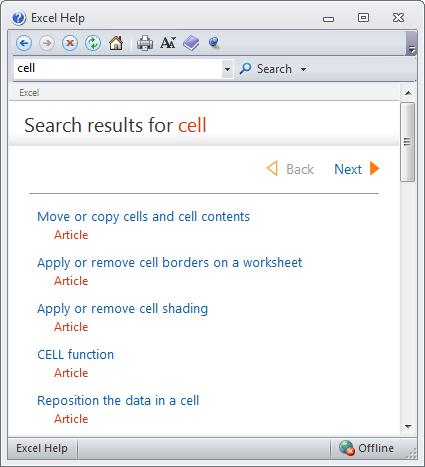
\includegraphics[scale=0.7]{../img/excel_2010_help.png}
\end{center}
\caption{Excel 2010 help.}
\label{img-excel_2010_help}
\end{figure}

